% 
%% Replace 'XX' with your paper number (assigned when you register abstract)
%% Replace 'NN' with actual number of pages. 

\documentclass[letterpaper,twocolumn,10pt]{article}
\usepackage{usenix2019,epsfig,subcaption}
%========================
%  Packages
%========================
%\usepackage{datetime}
\usepackage{url}
%\usepackage{hyperref}
\usepackage{color}
%\usepackage{graphicx}
\usepackage{algorithm}
\usepackage[noend]{algpseudocode}

%========================
%  Macros
%========================

\newcommand{\code}[1]{\textsf{\fontsize{9}{11}\selectfont #1}}

\newcommand{\inred}[1]{{\color{red}{#1}}}
\newcommand{\remove}[1]{}
\newcommand{\Idit}[1]{\inred{[Idit: #1]}}

\newcommand{\sys}{YoDB}

\newcommand{\tuple}[1]{\ensuremath{\langle \mbox{#1} \rangle}}

\usepackage{cleveref}


\crefformat{section}{\S#2#1#3}




% No date in title area.
\date{}


% Actual document begins below.
\begin{document}

\title{\sys\ -- Supplementary Material} 
\author{}
\maketitle

\section{Chunk Structure}
The chunk metadata structure is given in Algorithm~\ref{alg:chunk}. 
The first field is its \emph{status}. 
It next holds a pointer to the appropriate funk, and either a munk or a Bloom filter, as well as a pointer to the next 
chunk in the chunk linked list.
Note that multiple \emph{generations} of munks may exist for a chunk throughout its life time.
Therefore the chunk metadata keeps the generation number of its latest munk, \code{gen}, and a per-generation \emph{sequence number},
\code{seq}, which is explained below. The chunk's \code{gen} and \code{seq} are stored together in one 64-bit word to allow 
atomic access to both of them. 
Finally, the chunk includes locks to synchronize concurrent access by multiple threads, as explained below.

\begin{algorithm}[htb]
\begin{algorithmic}
\State \code{status} \Comment  baby, child, active, immutable, or aged
\State ptr \code{funk} \Comment funk disk address
\State ptr \code{munk} \Comment munk memory pointer
\State ptr \code{next} \Comment next chunk in linked list
\State int \code{gen} \Comment munk generation
\State int \code{seq} \Comment sequence number in current generation 
\State ptr \code{bloomFilter} \Comment summary of set of keys in \code{log}
\State asymmetric lock \code{rebalanceLock} \Comment shared/exclusive lock 
\State lock \code{funkChangeLock} \Comment acquired with try\_lock 
\State \code{PPA[threads]} \Comment pending puts
\end{algorithmic}
\caption{Chunk metadata structure.}
\label{alg:chunk}
\end{algorithm}

\section{Synchronization Data Structures}
Using a single pending array to synchronize all
operations can cause unnecessary contention.
We mitigate this problem in our implementation by maintaining two data structures for coordinating different operations. The first is a per-chunk pending put array (\emph{PPA}) which 
either indicates the current update's key and version, or indicates that the thread is currently not performing a put.
%maps each thread either to a cell in the chunk that the thread is currently attempting to put into and a corresponding version, or an indication that the thread is currently not performing a put. 
The second is a global pending scan array (\emph{PSA}) which tracks versions used by pending scans for compaction purposes; each entry consists of a version and a sequence number, as well as the scan’s key range. Each entry in the \code{PPA}s and \code{PSA} includes, in addition to the operation metadata, an ABA sequence number. 

A put operation consists of 5 phases: 
\begin{enumerate}\itemsep0pt
\item \emph{pre-process} - locate the target chunk; if a munk exists, prepare a cell to insert the value into; 
\item \emph{publish} - obtain a version while synchronizing with concurrent scans and rebalances via the chunk's lock and publish indication in the chunk's \code{PPA}; 
\item \emph{persist} - write the data into the log, indicate it is persisted in the \code{PPA}; 
\item \emph{link} - if a munk exists, connect the new cell to the linked list, so it can be found through the list traversal, otherwise, update the row cache to latest version if key is present in the cache; and finally
\item \emph{clean} - clear the entry in the chunk's \code{PPA}, and increase the entry's ABA number.
\end{enumerate}

If the put fails to acquire the chunk's lock (since it is being rebalanced), the operation restarts, and re-attempts to find an active chunk.
Puts trigger both munk and funk rebalances. The former are handled inline when the munk is close to overflow; the latter are done in the background 
by helper threads.

A per-chunk linearization counter is used to determine the order of concurrent put operations updating the same key.  
%Note that multiple \emph{generations} of munks may exist for a chunk throughout its life time.
Therefore, the linearization counter is composed of three parts: (a) the GV value; (b) \code{gen} - incremented whenever a munk is cached into memory and when the munk is rebalanced; and (c) \code{seq} - incremented upon each put and set to the number of KV-pairs in a munk upon a new generation number. When a new chunk is created as a result of a split, the children chunks inherit their generation number from their parent. The linearization counter is written both to the \code{PPA} upon publishing the put operation, and to the \code{log} when persisting the data. This ensures all operations see the same order of writes per key.

A scan operation first publishes its intent to obtain a version in the \code{PSA}. It determines its scan time $t$ by increasing GV and writing it to its entry in the \code{PSA}. The scan operation then starts traversing the chunks in its range. For each chunk, it first waits for all put operations that are either with smaller version than $t$ or still have not acquired a version to clear their entry in the \code{PPA} or acquire a larger version. After waiting for all concurrent puts to complete, the scan  can read the range from the chunk. If a munk exists, it simply reads the range from the linked list, skipping versions that are not last before $t$. Otherwise, the scan merges the \code{SSTable} and \code{log} data and reads the range from the result, again skipping the penultimate versions. When the scan completes, it clears the entry in the \code{PSA}, and increases the entry's ABA number. Get operations access neither the \code{PSA} nor the \code{PPA}.% data structures.

A munk rebalance iterates through the \code{PSA} to collect the maximum version number among the active scans that cannot be reclaimed yet. If a scan published its intent in the \code{PSA} but published no version number yet, the rebalance waits until either the version is published or the ABA number in the entry is increased. 

\section{Supplmental Evaluation Results}

\subsection{Get-Dominated Workloads}

Figure~\ref{fig:gets} presents the throughput result for get-dominated workloads.   
We see that YCSB-B (5\% put, 95\% get, Figure~\ref{fig:throughput:b}) achieve results similar  to YCSB-C (100\% get) that was presented in the main paper.
Namely, \sys\/ achieves up to $1.6$x throughput versus RocksDB both with composite keys and with simple ones.   

For completeness, we also experimented with the standard YCSB  \emph{Latest-simple} distribution.
In workload YCSB-D (5\% put, 95\% get) keys are inserted in sequential order; the read keys' distribution is skewed towards recently added ones. 
Specifically, the sampled key's position wrt the most recent key is distributed Zipf. This is a 
workload with medium spatial and temporal locality that represents, e.g., status updates and reads. Throughput results are depicted in Figure~\ref{fig:throughput:d}.

\begin{figure*}[tb]
\centering
\begin{subfigure}{0.45\linewidth}
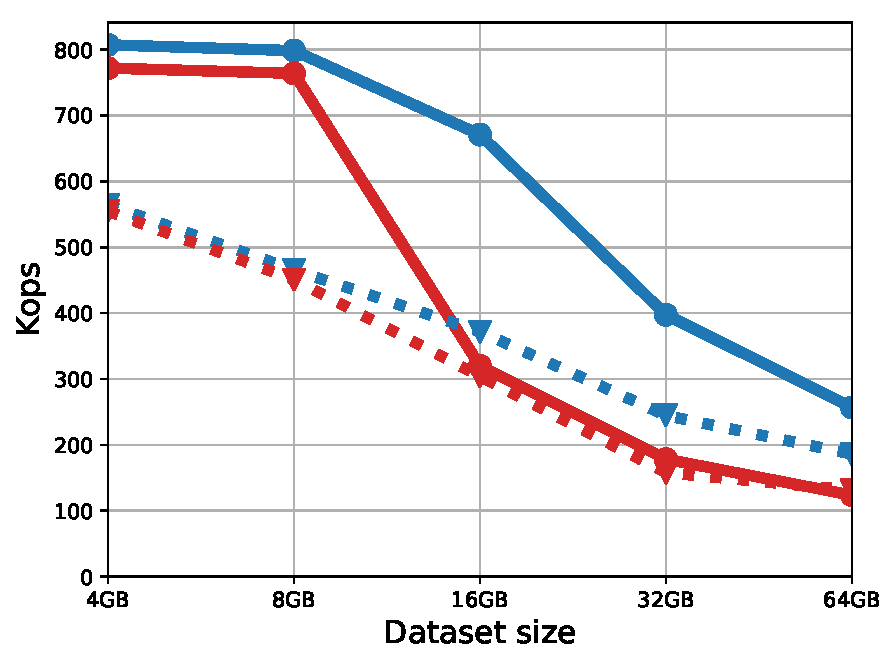
\includegraphics[width=\textwidth]{figs/Workload_B_line.pdf}
\caption{YCSB-B}
\label{fig:throughput:b}
\end{subfigure}
\begin{subfigure}{0.45\linewidth}
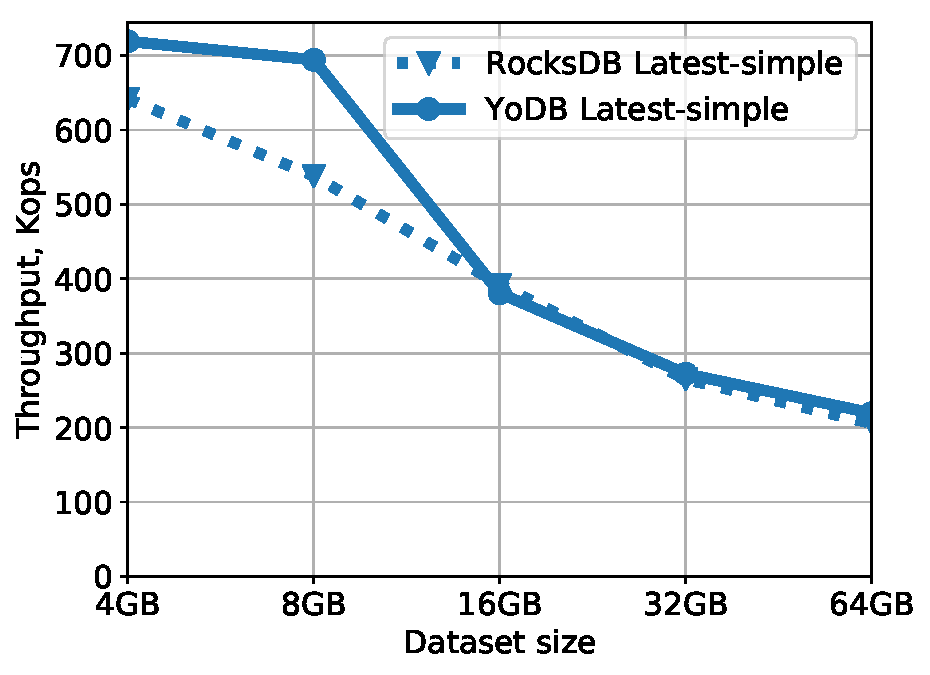
\includegraphics[width=\textwidth]{figs/Workload_D_line.pdf}
\caption{YCSB-D}
\label{fig:throughput:d}
\end{subfigure}
\caption{
{\sys\/ versus RocksDB throughput (Kops), under get-dominated workloads with Zipf distributions over composite (two-component) and
simple (non-composite) keys and scaling dataset sizes.}
}
\label{fig:gets}
\end{figure*}

\subsection{Scan-Dominated Workloads}
In addition to experimenting with the default maximum \code{log} size (2MB), we also experimented with smaller \code{log}s (256KB maximum size).
Figure~\ref{fig:scans} presents the throughput result for scan-heavy workloads (YCSB-E) with three different scan 
sizes. It can be seen that with Zipf-simple distribution over large data sets \sys\ scans benefit from smaller \code{log}s as mergeing them with SSTables is faster.

\begin{figure*}[tb]
\centering
\begin{subfigure}{0.33\linewidth}
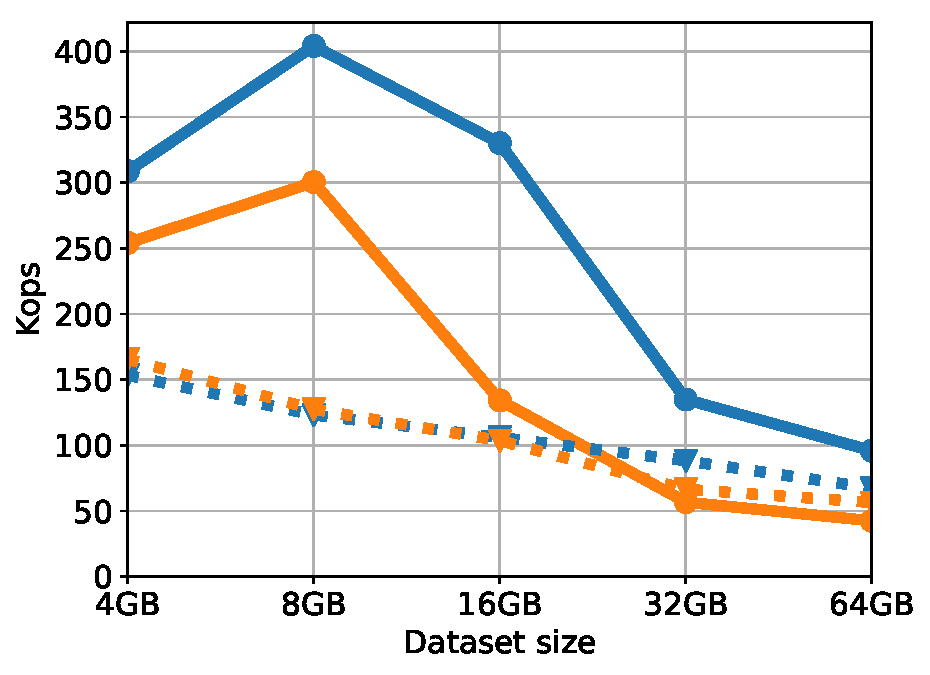
\includegraphics[width=\textwidth]{figs/complementary/Workload_E-_line.pdf}
\caption{YCSB-E10 -- short scans}
\label{fig:throughput:e10}
\end{subfigure}
\begin{subfigure}{0.33\linewidth}
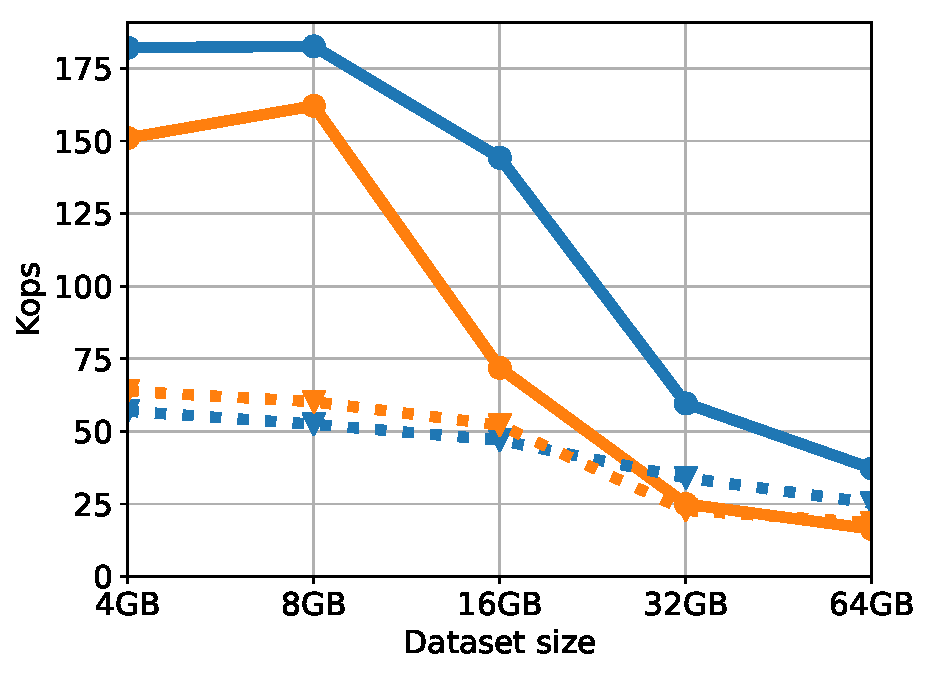
\includegraphics[width=\textwidth]{figs/complementary/Workload_E_line.pdf}
\caption{YCSB-E100 -- medium scans}
\label{fig:throughput:e100}
\end{subfigure}
\begin{subfigure}{0.33\linewidth}
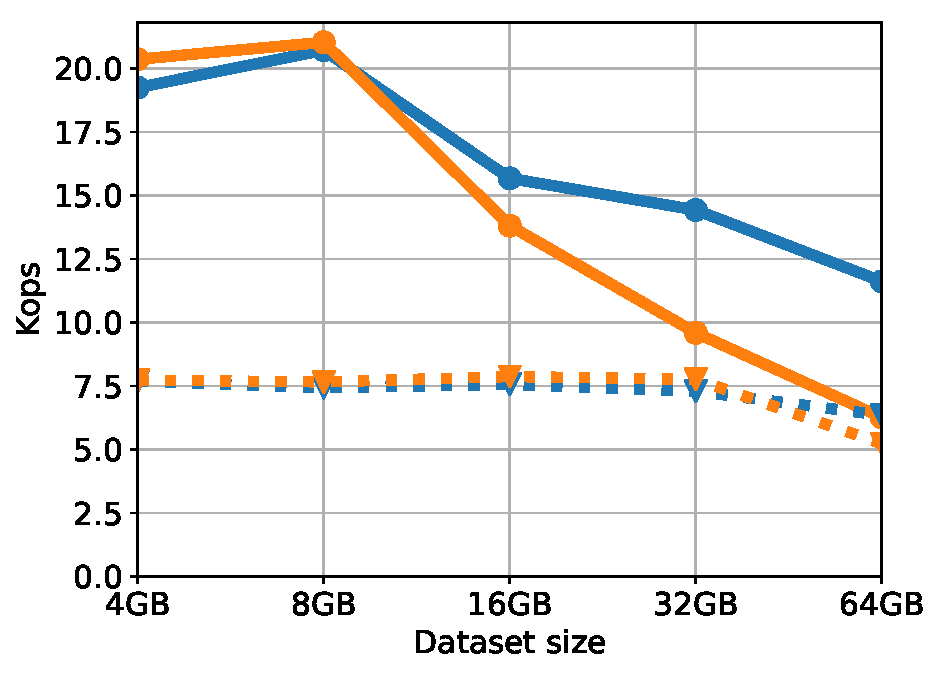
\includegraphics[width=\textwidth]{figs/complementary/Workload_E+_line.pdf}
\caption{YCSB-E1000 -- long scans}
\label{fig:throughput:e1000}
\end{subfigure}
\begin{subfigure}{\linewidth}
\centerline{

\includegraphics[width=0.9\textwidth]{figs/legend.pdf}
\vspace{-5mm}
}
\end{subfigure}
\caption{
{\sys\/ versus RocksDB throughput (Kops), under scan-dominated workloads with Zipf distributions over composite (two-component) and
simple (non-composite) keys and scaling dataset sizes.}
}
\label{fig:scans}
\end{figure*}



\end{document}
